%% sections/introduction.tex
\section{Introduction}\label{introduction}

Dong drum towers are among the most representative public timber
structures in traditional Dong villages in Southwest China, particularly
in Guizhou, Hunan, and Guangxi. As architectural landmarks and communal
infrastructures, they embody the regional identity, social organization,
construction knowledge, ritual life, and collective memory of Dong
communities. Typically constructed from Chinese fir or other locally
treated timber, drum towers are assembled through mortise-and-tenon
joints without the use of nails or metal fasteners, forming compact,
durable, and highly hierarchical wooden structures. Their elevated
columns, interlocking beams, layered eaves, roof-crown systems, and
tiered supporting frameworks reflect the craftsmanship and structural
ingenuity of Dong master carpenters. Historically, drum towers served as
central public spaces for village assemblies, covenant making, warning
against external threats, festive gatherings, musical performance, and
intergenerational cultural transmission. Their architectural form is
therefore not merely a physical construction, but a material carrier of
community practice, craft knowledge, spatial order, and intangible
cultural heritage.

Previous studies have examined Dong drum towers from multiple
perspectives, including construction techniques, structural typologies,
regional distribution, roof-crown systems, bracket components, and
master-carpenter knowledge, thereby establishing a fundamental
architectural understanding of this distinctive timber heritage type
[1--5]. At the settlement scale, further research has shown that
drum towers are closely embedded in the spatial organization, cultural
transformation, and design preferences of Dong villages [6,7]. These
studies demonstrate that drum towers should be understood as both
technical timber structures and socio-cultural infrastructures. As shown
in Fig. 1, their morphological characteristics, including eave
hierarchy, roof type, plan configuration, tower height, and crown form,
reveal substantial diversity across different villages and construction
traditions.

\begin{figure}[htbp]
    \centering
    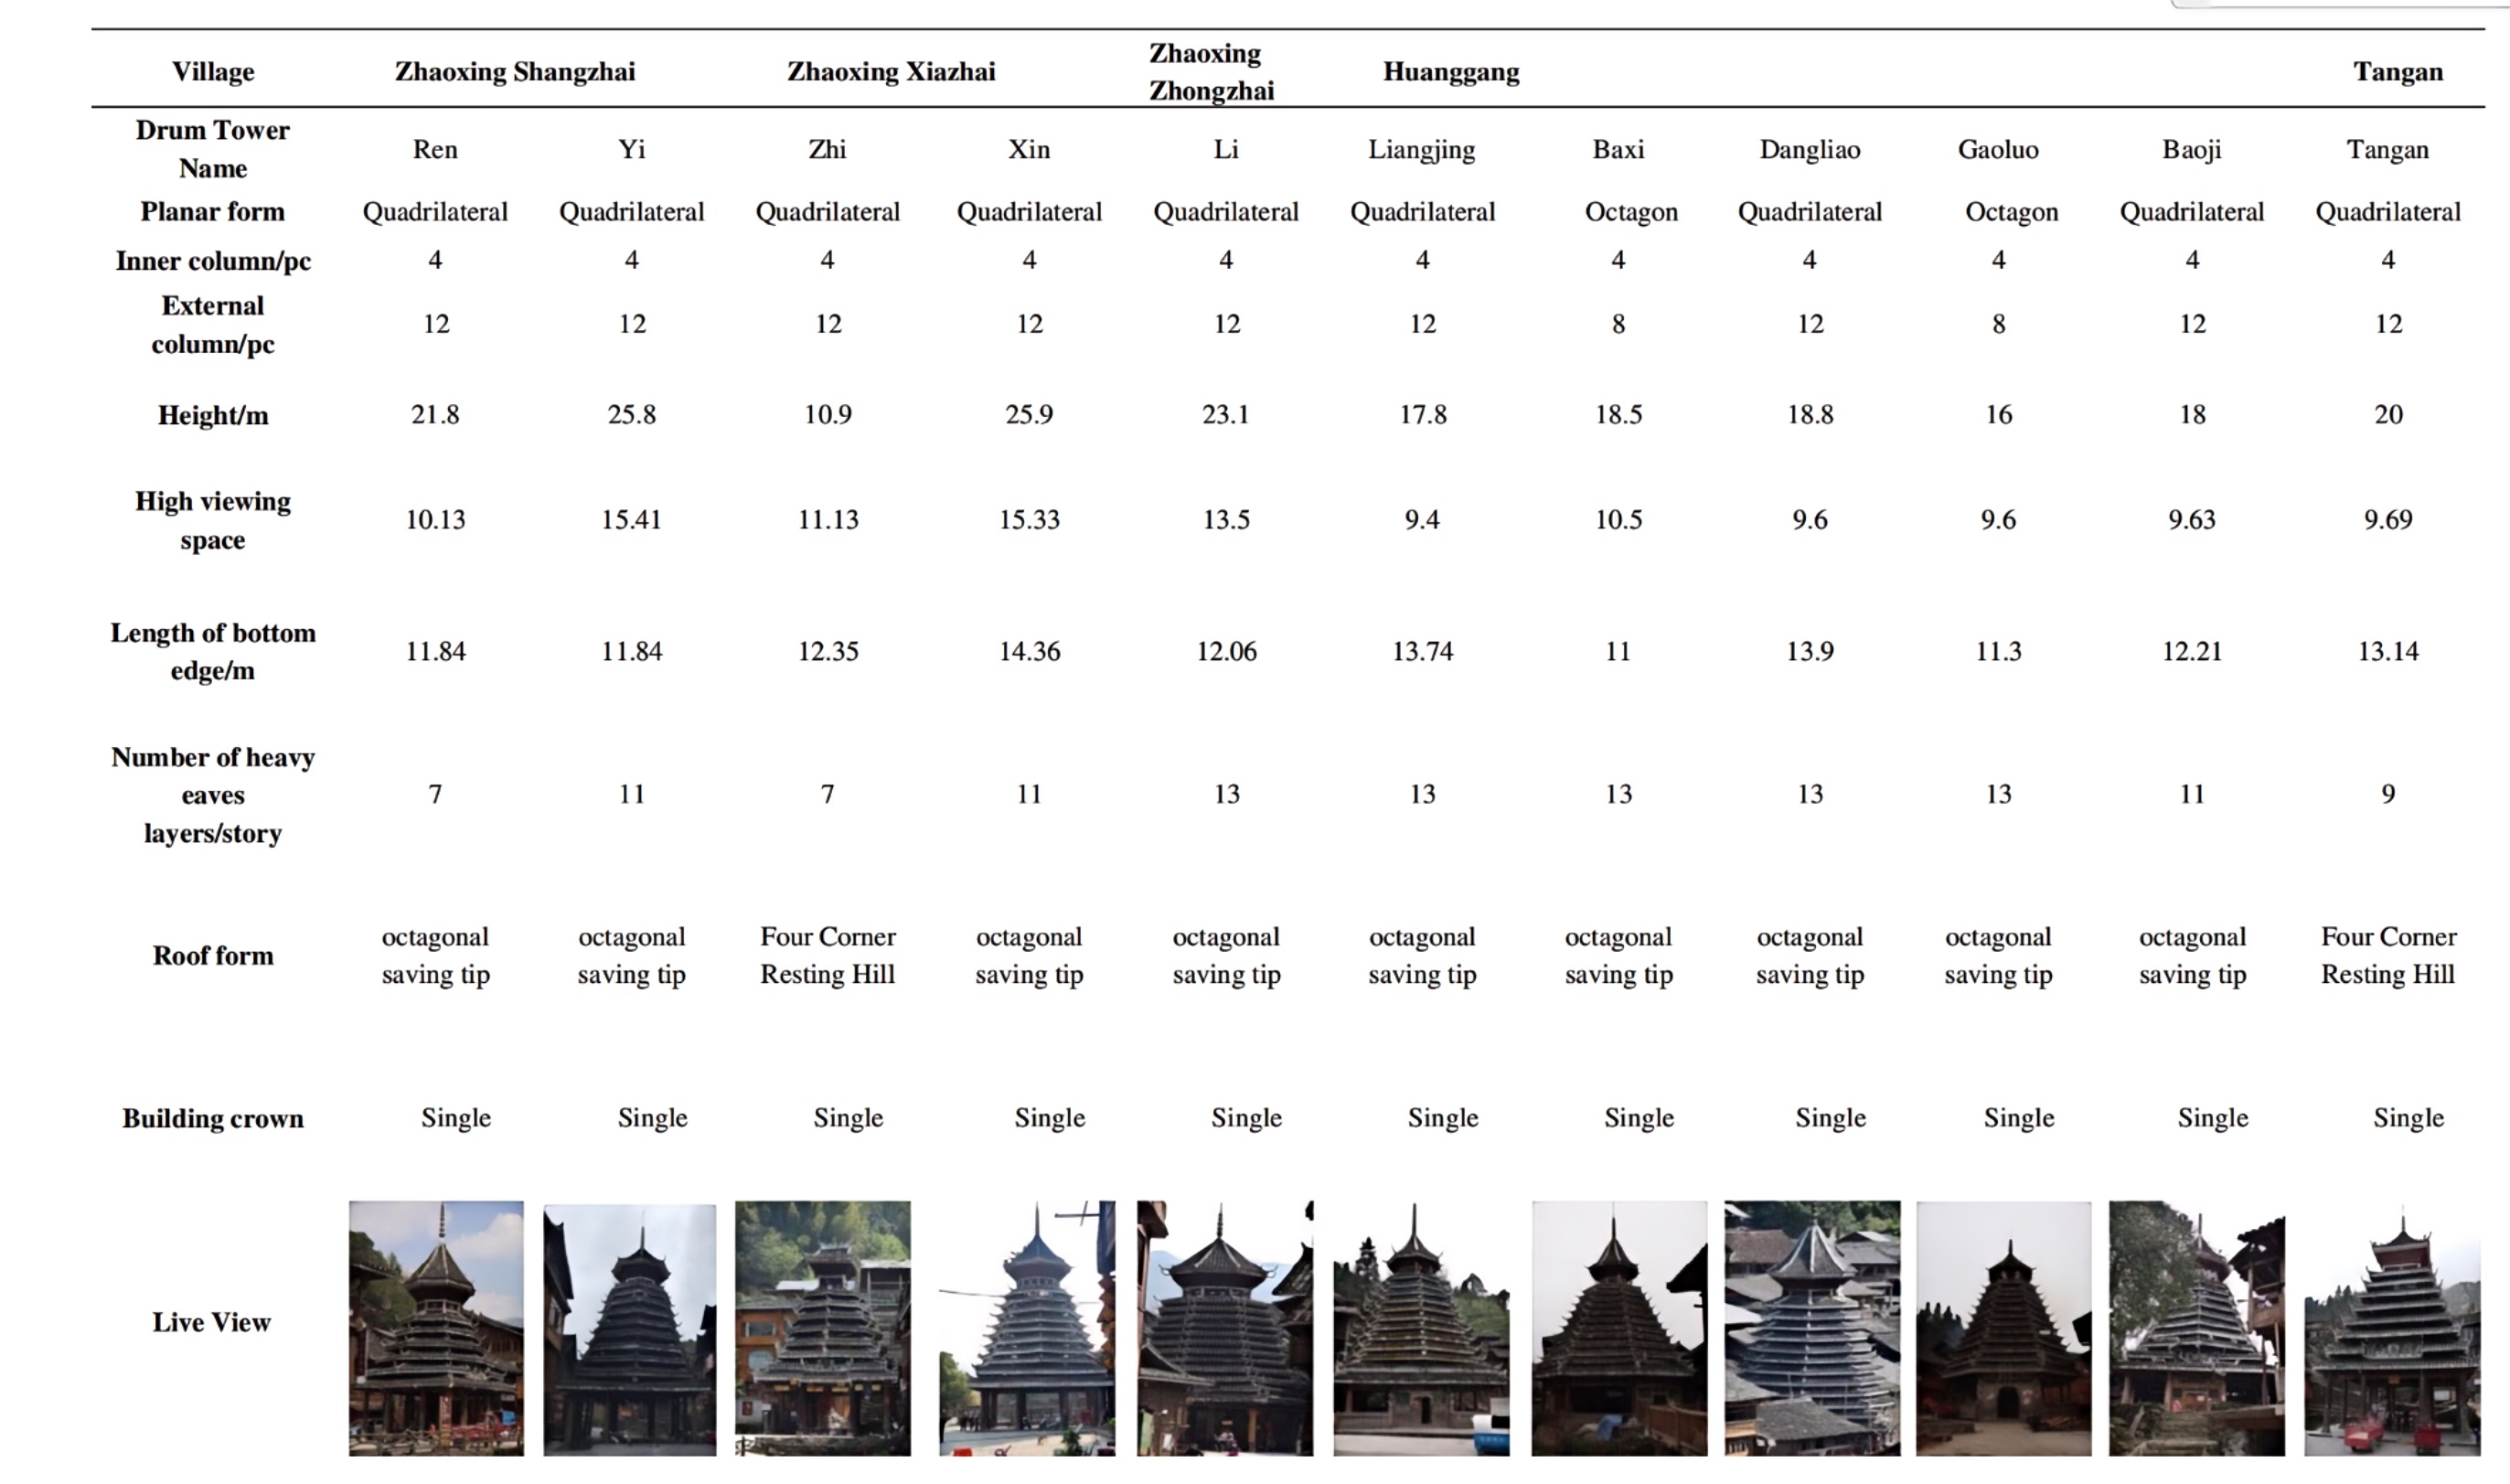
\includegraphics[width=\linewidth]{figures/media/image1}
    \label{fig:pandoc_1}
\end{figure}


\begin{figure}[htbp]
    \centering
    \includegraphics[width=\linewidth]{figures/media/image2}
    \label{fig:pandoc_2}
\end{figure}


\textbf{Fig. 1. Morphological characteristics and spatial forms of
representative Dong drum towers[8].}

Recent scholarship has extended Dong drum tower research from
architectural description to digital heritage, acoustic simulation,
mathematical metamodeling, UAV-based reconstruction, and intelligent
heritage building information modeling. Mao et al. demonstrated that the
spatial form of Dong drum towers is closely associated with sound-field
characteristics and ceremonial use [9]. Deng et al. proposed
mathematical metamodeling for automated simulation of Dong drum tower
architectural heritage, highlighting the possibility of computational
representation of traditional timber structures [10]. Huang et al.
developed a digital preservation workflow for endangered Dong drum
towers by integrating field investigation, UAV documentation, BIM, and
3D reconstruction [11]. Deng et al. further introduced an
intelligent HBIM framework that combines machine vision and
architectural expertise for traditional timber heritage, validating its
applicability using Dong drum tower data [12]. Related studies on
Dong soundscapes and traditional village morphology also indicate that
Dong architectural heritage should be understood as a coupled system of
built form, spatial organization, acoustic experience, and community
practice [13--15].

From the perspective of heritage science, the documentation of Dong
drum towers requires more than geometric recording or visual
reproduction. International heritage frameworks have emphasized the
protection of intangible cultural practices, authenticity, and wooden
built heritage [16--18]. For timber architecture in particular,
conservation-oriented documentation must support the understanding of
material condition, structural configuration, component relationships,
construction logic, and long-term maintenance needs [19]. Digital
documentation technologies have therefore become increasingly important
in architectural heritage conservation. HBIM has been widely adopted to
connect geometric documentation, semantic information, conservation
records, and heritage management workflows [10--24]. In parallel,
photogrammetry, 3D scanning, and image-based recording techniques have
provided robust technical foundations for capturing complex heritage
morphology [25--27]. However, for highly layered timber structures
such as Dong drum towers, the central challenge is not only whether a
digital model can be generated, but whether conservation-relevant
components can be faithfully recovered, interpreted, and used for
downstream heritage tasks.
